\chapter{Evaluation}
\label{chap:evaluation}

Five experiments were performed to validate the functionality of the tags.
The first is non specific and ment to test the setup in a stable environment.
Experiments two to four are intended to test the detection of unwanted circumstances.
Experiment five is tests the system in a real-world environment.
The experiment results were stored on the phone and then exported using email.
The analysis of the data and creation of graphs was then performed using a Jupiter Notebook, using Pandas and Pyplot for datamanagment and the creation of graphs.\\
For all experiments the query-frequency was set to 330s.
The measurements queries are spread across this timeframe.
Each experiment lasted between 40 minutes and one hour.
All eperiments were performed two to three times.
In each section only the data-set from the first experiment run is presented fully.
The other experiments will be mentioned only, if they have differing data or to confrim an unexpected datapoint.

The tags used were programmed as described in Chapter \ref{c:implementation}.
The same four tags were used for all experiments.
They will be refered to as Tag-1, Tag-2, Tag-3 and Tag-4.





\section{Experiment 1: Static}
\label{ss:exp_1}
The four tags where placed on the corners of a 80 cm by 50 cm rectangle on a wooden table.
Figure \ref{f:exp1_schematic} shows a schematic view of the setup.
Each tag was turned on sequentially and given enough time to establish the network.
The phone then was connected to Tag-4.
The parameters in the app were left unchanged.
The default parameters are large enough, that no measurement should be able to trigger a warning.
Orientational reading was used for the output of the gyroscope.
The setup was then left untouched for 35 min.
The goal of this experiment was, to gauge by how much the measurements can vary in a static environment.

\begin{figure}[ht!]
	\centering
	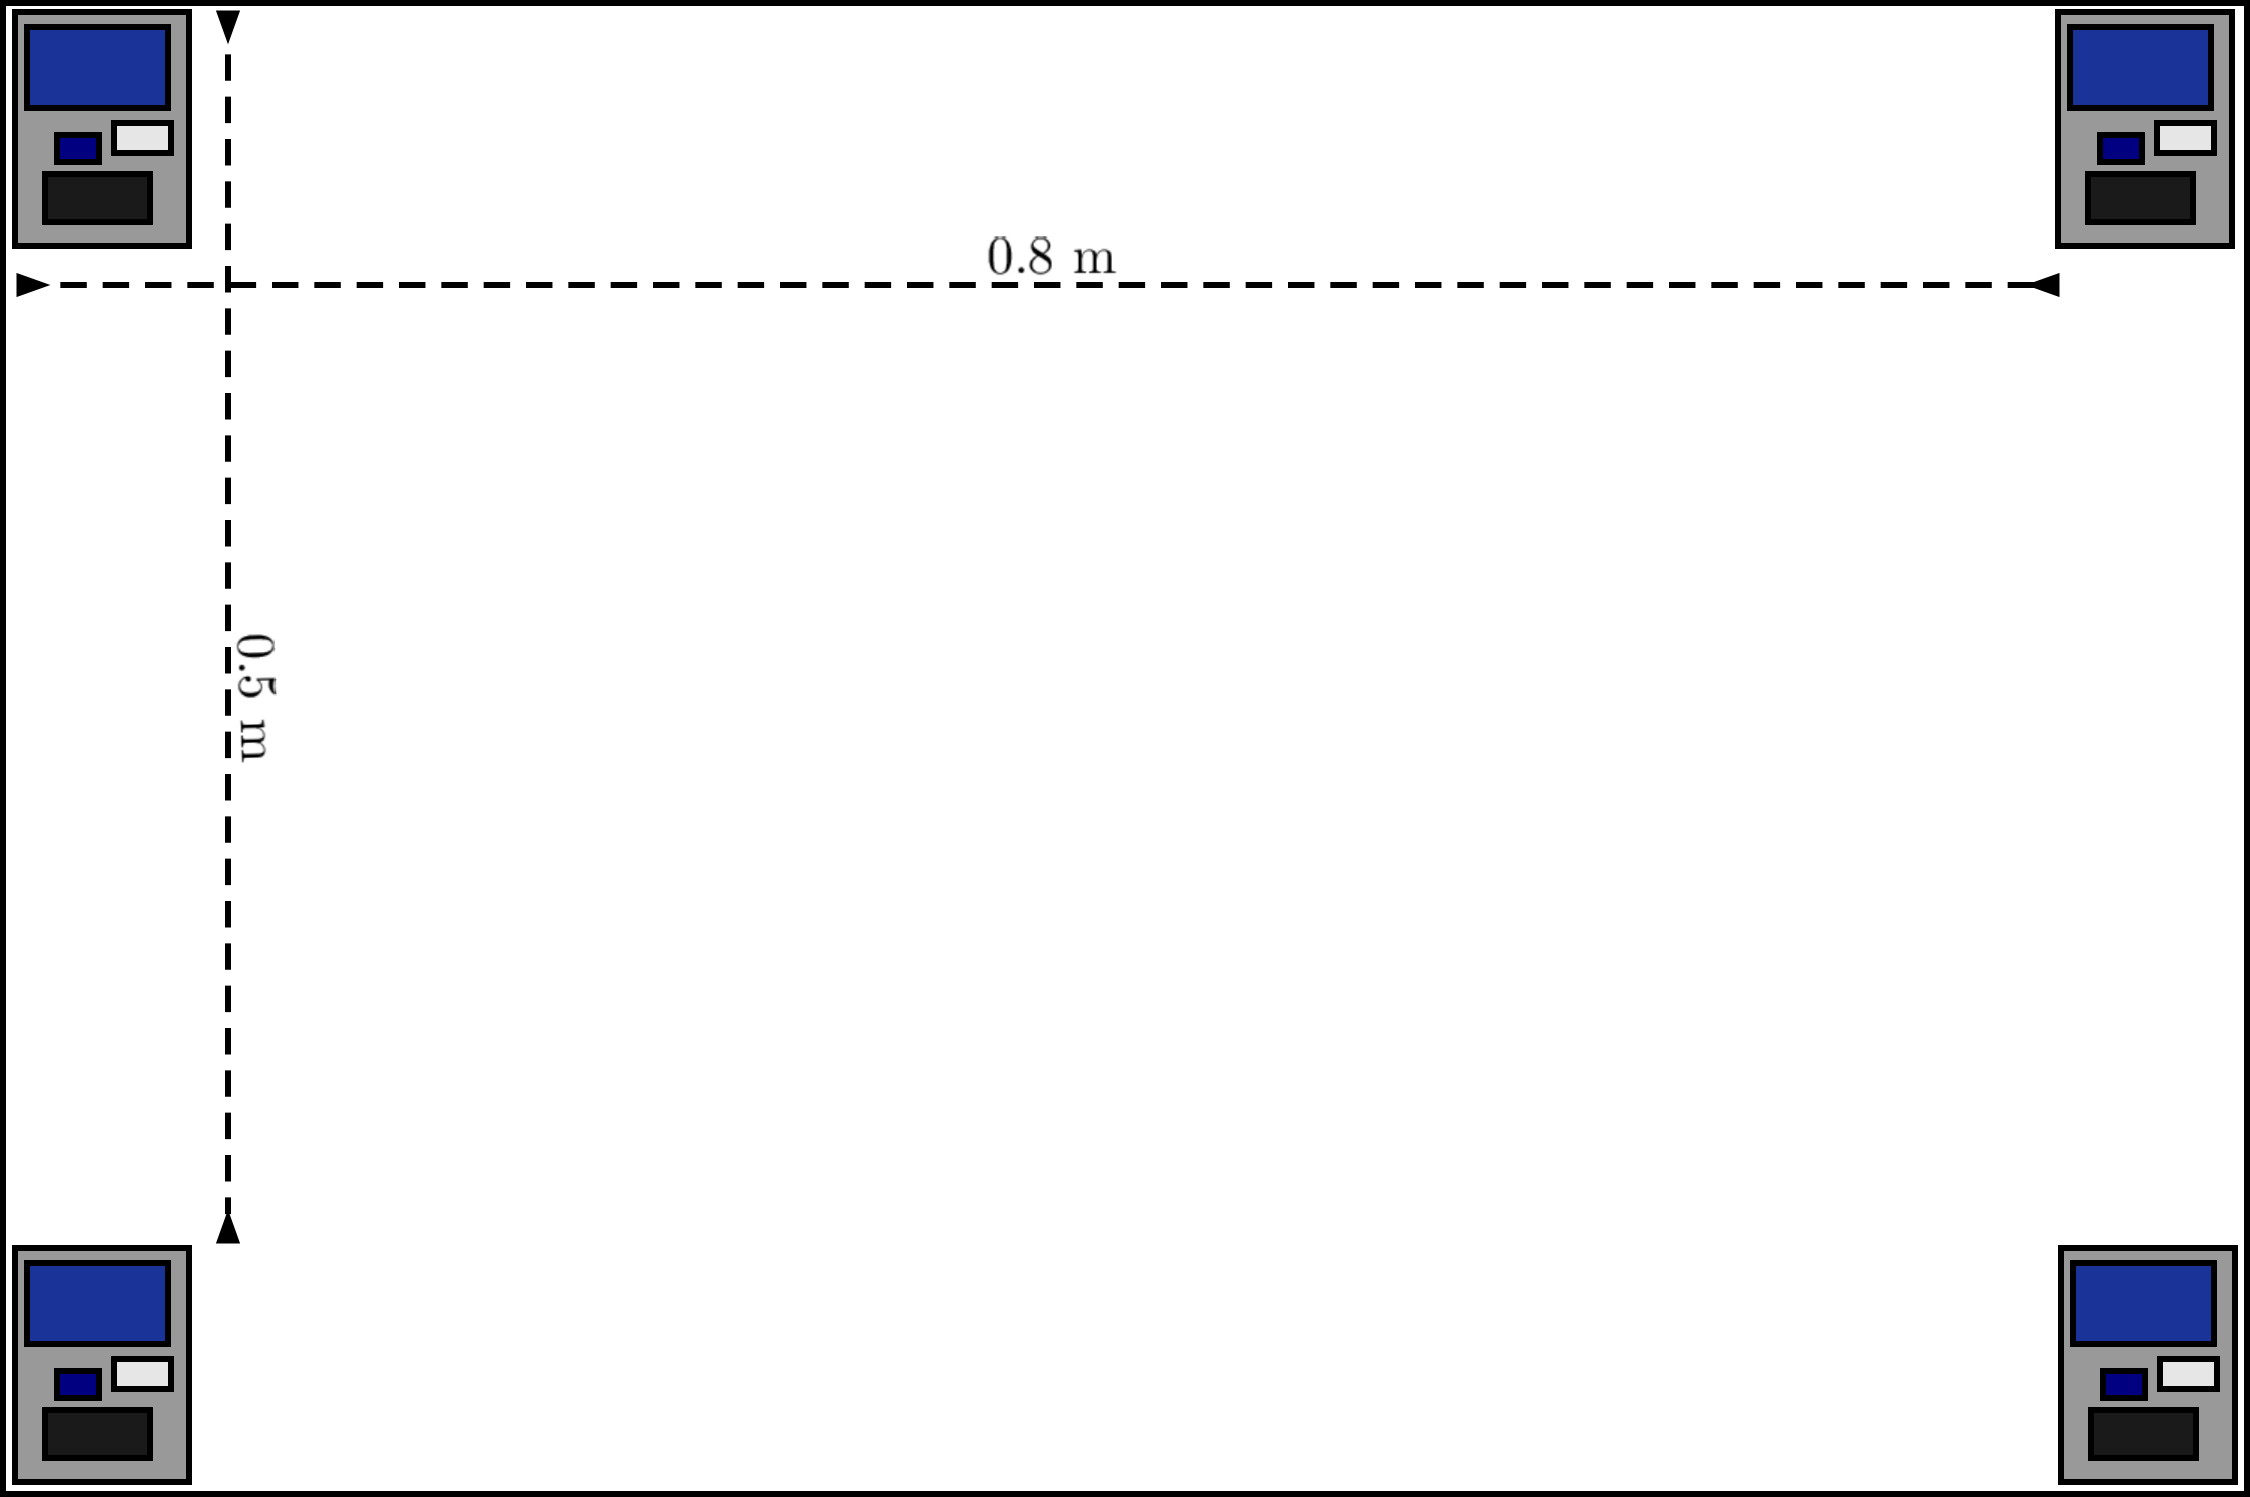
\includegraphics[width=300px]{graphics/schematics/experiment_1.png}
	\caption{Schema of the setup of experiment 1.}
	\label{f:exp1_schematic}
\end{figure}


\subsection{Results}
\label{ss:exp_1_result}
In eperiment one, all measurements are expected to be unchanging.
Table \ref{t:exp1_means} shows the mean values for temperature, humidity and angle during the experiment by tag.
Figures \ref{f:exp1_graphs_temp}, \ref{f:exp1_graphs_hum}, \ref{f:exp1_graphs_gyro}, \ref{f:exp1_graphs_dist} shows the change of these values over time.

\begin{table}[ht]
\centering
\caption{Mean and Variances for Temperature and Humidity Data by Tag during experiment 1.}
\begin{minipage}{0.45\textwidth}
\centering
	\begin{tabular}{|c|c|c|}
		\hline
		\textbf{Tag} & \textbf{Temp} & \textbf{Hum} \\
		\hline
		Tag-1 & 22.06 & 32.56 \\
		Tag-2 & 21.90 & 33.93 \\
		Tag-3 & 22.06 & 32.94 \\
		Tag-4 & 21.87 & 32.80 \\
		\hline
	\end{tabular}
	\caption*{Mean}
\end{minipage}
\hfill
\begin{minipage}{0.45\textwidth}
\centering
	\begin{tabular}{|c|c|c|}
		\hline
		\textbf{Tag} & \textbf{Temp} & \textbf{Hum} \\
		\hline
		Tag-1 & 0.02 & 0.03 \\
		Tag-2 & 0.05 & 0.04 \\
		Tag-3 & 0.03 & 0.06 \\
		Tag-4 & 0.03 & 0.05 \\
		\hline
\end{tabular}
\caption*{Variance}
\end{minipage}
\label{t:exp1_means}
\end{table}

\begin{figure}[ht!]
	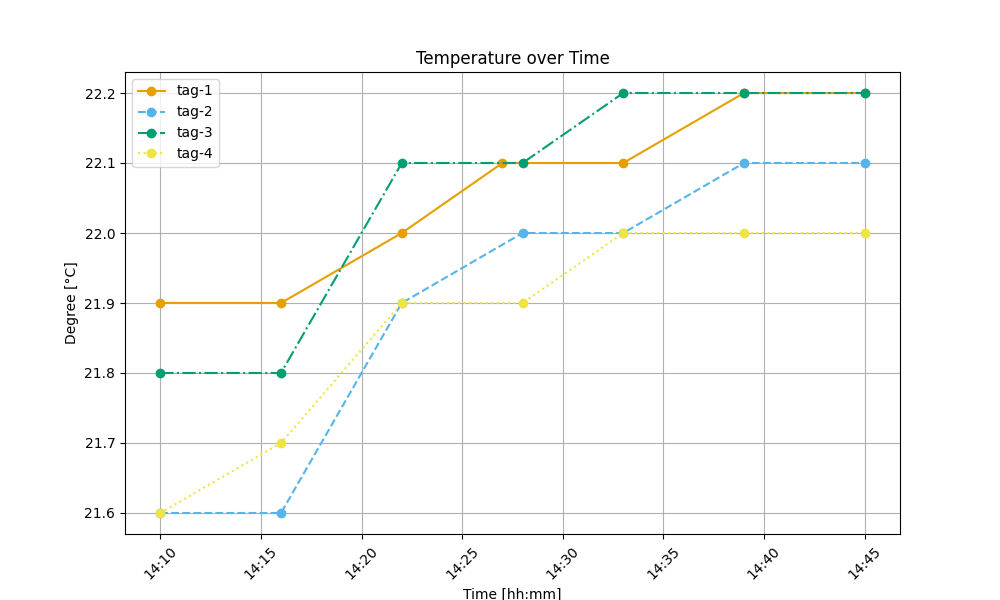
\includegraphics[width=\linewidth]{graphics/exp/exp1_temp_plot_0.png}
	\caption{Experiment 1, temperature over time.}
	\label{f:exp1_graphs_temp}
\end{figure}

Figure \ref{f:exp1_graphs_temp} shows the recorded temperature during experiment 1.
The tags are color coded and use different line-styles.
To make it easier to distinguische the lines, the Y axis only displayes the relevant section, rather then starting at 0\degree .
The time at the bottom represents the timestamp at which the measurement arrived at the phone.
All four tags have a mean temperature between 21.8 and 22.1 \degree C.
The varaince are also small, tag two having the highest one with 0.05 \degree C variance. 
The graph shows that all tags have a rising temperature.
The increase is quite small with tag two having the biggest increase of 0.5 \degree C over 20 minutes.
When the experiment was repeated,, the means stayed similar between the tags and the variance became only smaller.
The trend in temperature changed from upwards to downwards, when the experiment was repeated.

\begin{figure}[ht!]
	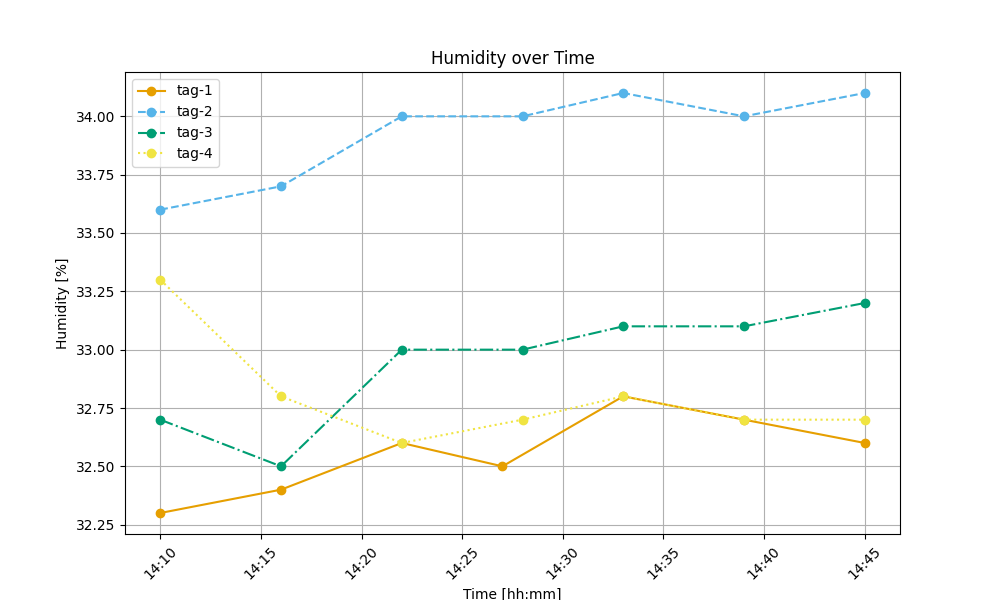
\includegraphics[width=\linewidth]{graphics/exp/exp1_hum_plot_0.png}
	\caption{Experiment 1, humidty over time.}
	\label{f:exp1_graphs_hum}
\end{figure}

Figure \ref{f:exp1_graphs_hum} shows the change of humidity over time.
Again, the relevant section of the y-axis is shown, rather than the full 0\% to 100\% , to increase readability.
The humidity of all sensor was similar as well.
The highest humidity was recorded by Tag-2 with 33.93\% .
Te lowest was recorded by Tag-1 with 32.56\% .
The variance is small, with Tag-3 having the biggest variance with 0.06\% pt.
During the first experiment, humidity increased by a small amount.
When the experiment was repeated,, the humidity dropped during the experiment.


\begin{figure}[ht!]
	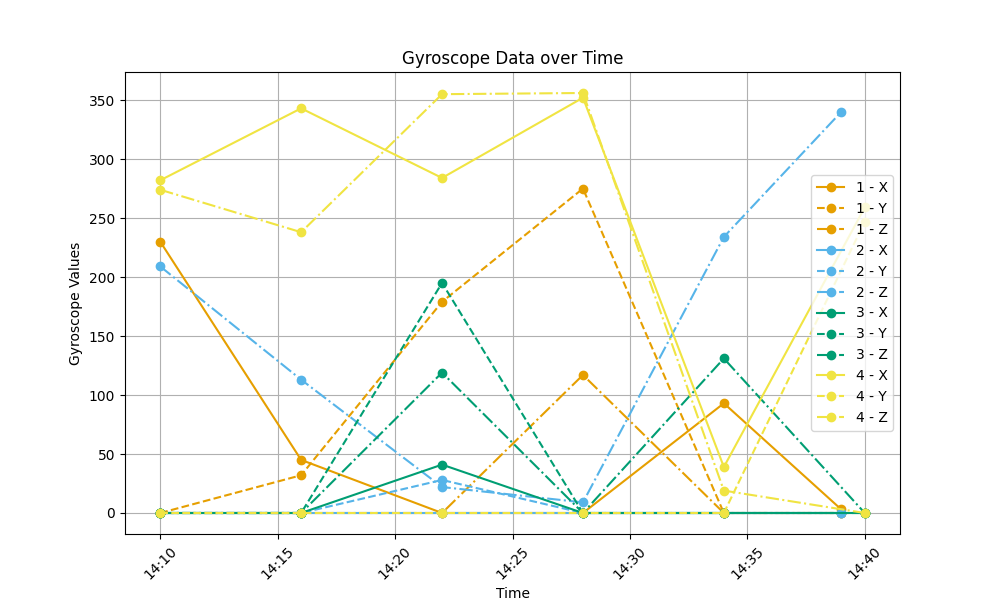
\includegraphics[width=\linewidth]{graphics/exp/exp1_gyro_data_plot_0.png}
	\caption{Registered value of the gyroscope over time during experiment 1.}
	\label{f:exp1_graphs_gyro}
\end{figure}

Since all tags were stationary during the experiment, the gyro sensor was expected to be unchanging.
This is not what occured.
The graph \ref{f:exp1_graphs_gyro} shows the values of the Gyroscope during experiment 1.
Orientational read was used, so the values shoud correspond to the angle around the given axis.
Each tag is assigned a color, and all angle measurements are shown in that color.
All X-axis measurement are diplayed using a filled line.
Axis-Y uses dotted lines.
Point-dotted lines represent the angles around axis-Z
Looking at the graph \ref{f:exp1_graphs_gyro} it is clear, that the measurement shows a wide range of angles for each tag and axis.
The angle of axis-X, Tag-1 (filled orange line) for example, jumps from a value of 230 \degree to 45 \degree, 0 \degree, then stays at 0 \degree for one measurement, goes up to 93 \degree and drops down again to 3 \degree.
As can be seen with this example is, that the measurements also don't fall a clear tragetory.
Tag-1 switches between rising and falling.
The only exception is tag 2 around the x axis, which stays at 0 for the whole measurement duration.\\
Since angle measurements fall into modular arithmetic, it "wrappes around" at 360\degree , means can only meanigfully be taken if the angles are in a small range.
Since this is not the case for most tags, the only mean that is meaningfull is tag 2 axis-x, which has a mean of 0 and a variance 0.

\begin{figure}[ht!]
	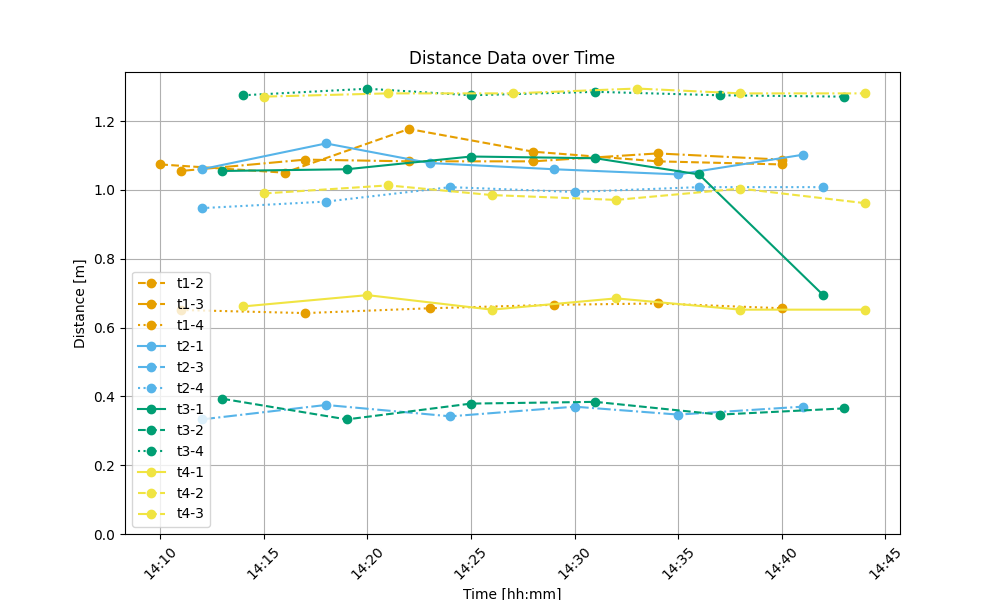
\includegraphics[width=\linewidth]{graphics/exp/exp1_dist_data_plot_0.png}
	\caption{Experiment 1, distance over time.}
	\label{f:exp1_graphs_dist}
\end{figure}

\begin{table}[ht]
\centering
	\caption{Mean, excpected values and variance of distant measurements, experiment 1.}
\begin{minipage}{0.45\textwidth}
	\begin{tabular}{|c|c c c c|}
		\hline
		& \textbf{Tag-1} & \textbf{Tag-2} & \textbf{Tag-3} & \textbf{Tag-4} \\
		\hline
		\textbf{Tag-1} & 0.0 & 1.094 & 1.084 & 0.657 \\
		\textbf{Tag-2} & 1.080 & 0.0 & 0.356 & 0.989 \\
		\textbf{Tag-3} & 1.007 & 0.367 & 0.0 & 1.279 \\
		\textbf{Tag-4} & 0.666 & 0.987 & 1.281 & 0.0 \\
		\hline
	\end{tabular}
	\caption*{Mean}
\end{minipage}
\hfill
\begin{minipage}{0.45\textwidth}
\centering
	\begin{tabular}{|c|c c c c|}
		\hline
		& \textbf{Tag-1} & \textbf{Tag-2} & \textbf{Tag-3} & \textbf{Tag-4} \\
		\hline
		\textbf{Tag-1} & 0.0 & 0.8 & 0.94 & 0.5 \\
		\textbf{Tag-2} & 0.8 & 0.0 & 0.5 & 0.94 \\
		\textbf{Tag-3} & 0.94 & 0.5 & 0.0 & 0.8 \\
		\textbf{Tag-4} & 0.5 & 0.94 & 0.8 & 0.0 \\
		\hline
	\end{tabular}
	\caption*{Excpected values}
\end{minipage}
\hfill
\begin{minipage}{0.45\textwidth}
	\centering
	\begin{tabular}{|c|c c c c|}
		\hline
		& \textbf{Tag-1} & \textbf{Tag-2} & \textbf{Tag-3} & \textbf{Tag-4} \\
		\hline
		\textbf{Tag-1} & 0.0 & 0.002 & 0.000 & 0.000 \\
		\textbf{Tag-2} & 0.001 & 0.0 & 0.000 & 0.001 \\
		\textbf{Tag-3} & 0.024 & 0.001 & 0.0 & 0.000 \\
		\textbf{Tag-4} & 0.000 & 0.000 & 0.000 & 0.0 \\
		\hline
	\end{tabular}
	\caption*{Variance}
\end{minipage}
\label{t:exp1_dist_var}
\end{table}

Table \ref{t:exp1_dist_var}, shows the mean, excpected value and variance of the measured distances.
The tag listed in the row is the queried tag that initiates the distance measurement, and the row corresponding to the responding tag.
By looking to the measurements diagonaly oposed to each other, one can see that the measured distaances is the the same, indipendent of who initiated the measurement, up to a range of two centimeters. 
The measurements from Tag-3 to Tag-1 is the highest, with 0.024m. All other variances are negibly small, beeing bellow 0.005m.
This shows that the measured distances are constant and stable, escept for the measurement from Tag-3 to Tag-1.
The distances measured do not correspond to the actual distances the tags had to each other, also seen in table \ref{t:exp1_dist_means}.
The measured distances can be as far of as 0.5 meters.
The two larger distances, 0.8 and 0.94 meters, correspond to the two larger measured values for each tag, while the smallest measured value always corresponds to the smallest distance, 0.5 meters.
The two larger values are not always ordered correctly, 0.94 meters sometimes beeing measured smaller then 0.8 meters.
In repeated experiments, all these facts stayed true.


Figure  \ref{f:exp1_graphs_dist} shows the measured distance over time.
A label i-j informe that tag-i initiated the measurement, and the distance between tag-i and tag-j was measured.
All measurements initiated by Tag-1 are orange. The meausrements of Tag-2 are blue, Tag-3 green and Tag-4 yellow.
The second tag that is involved in the measurement is signified by the line.
Measurements to Tag-1 use filled lines. Measurements to Tag-2 use dashed lines, Tag-3 uses dashed and dotted lines and Tag-4 uses dotted lines.\\
All lines except for 3-1 are horizontal  and show little variance.
Measurement 3-1 is also stable untl the last measurement, where a datapoint that is 0.35m lower than all previously recorded data is measured.
One can also see that not all measurements start at the same time.
The first measurement of distance 1-2 was registered at 14.10, while the first measurement of 4-3 was recorded at 14.15.
Each distance was measured seven times and with equidistance measurement times.

\begin{figure}[ht!]
	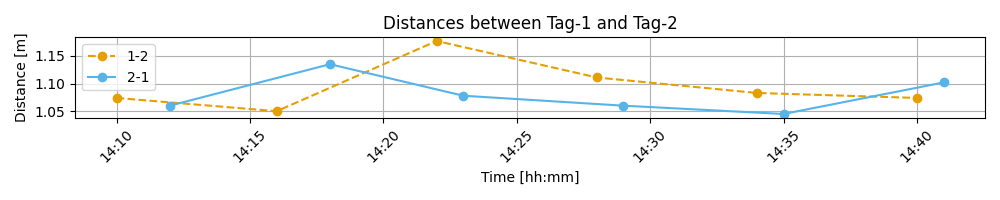
\includegraphics[width=\linewidth]{graphics/exp/exp1_dist_data_plot_1_1_2_split.png}
	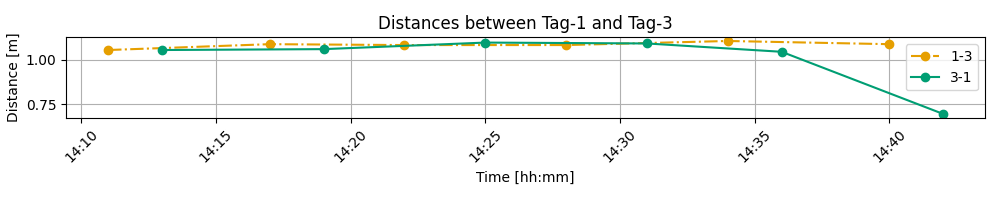
\includegraphics[width=\linewidth]{graphics/exp/exp1_dist_data_plot_1_1_3_split.png}
	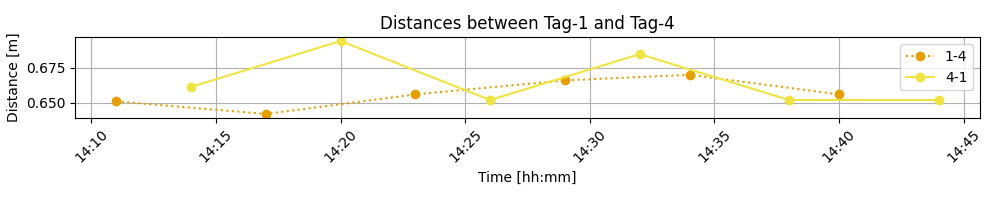
\includegraphics[width=\linewidth]{graphics/exp/exp1_dist_data_plot_1_1_4_split.png}
	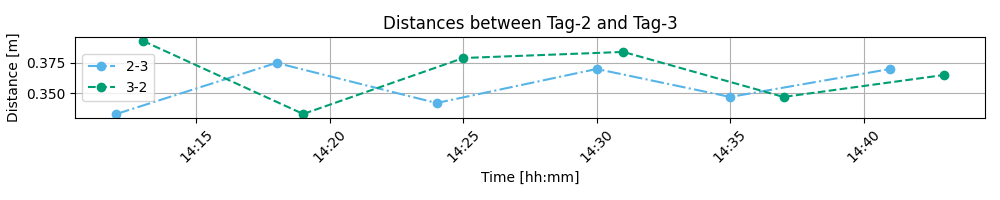
\includegraphics[width=\linewidth]{graphics/exp/exp1_dist_data_plot_1_2_3_split.png}
	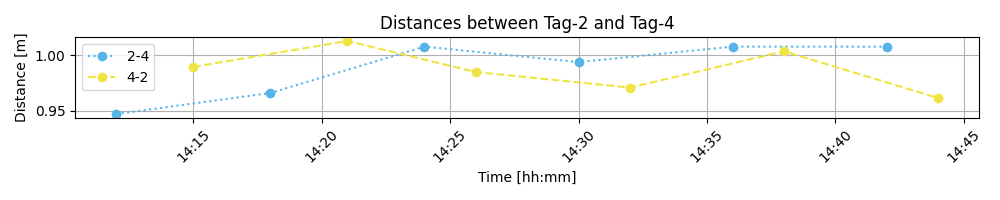
\includegraphics[width=\linewidth]{graphics/exp/exp1_dist_data_plot_1_2_4_split.png}
	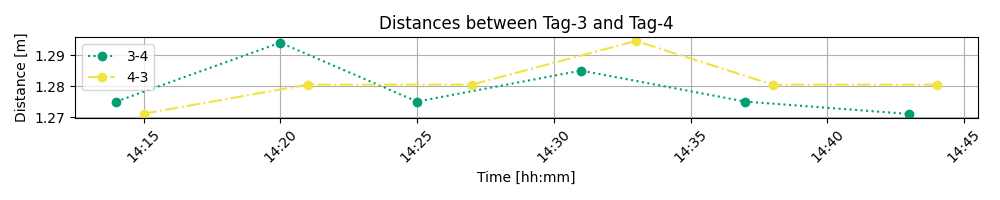
\includegraphics[width=\linewidth]{graphics/exp/exp1_dist_data_plot_1_3_4_split.png}
	\caption{Experiment 1, distance over time, for all pairs i-j.}
	\label{f:exp1_graphs_dist_split}
\end{figure}


The measurement pairs i-j and j-i report the same distance, but with different tags initiating the measurement. 
To better compare these pairs, figure \ref{f:exp1_graphs_dist_split} shows six subplots of figure \ref{f:exp1_graphs_dist} containing only each of these pairs.
The graphs show that the measurement pairs anre consistently close together.
One outlier happens when Tag-3 measures the distance to Tag-1 at very end of the measurements.
The measured value drops 0.35m bellow the previous mean of 1.30m.
When repeating this experiment and during other experiments, these outliers happened again, a bit less frequently then twice per hour.
The outliers always affected a measurement involving tag 1.

\begin{figure}[ht!]
	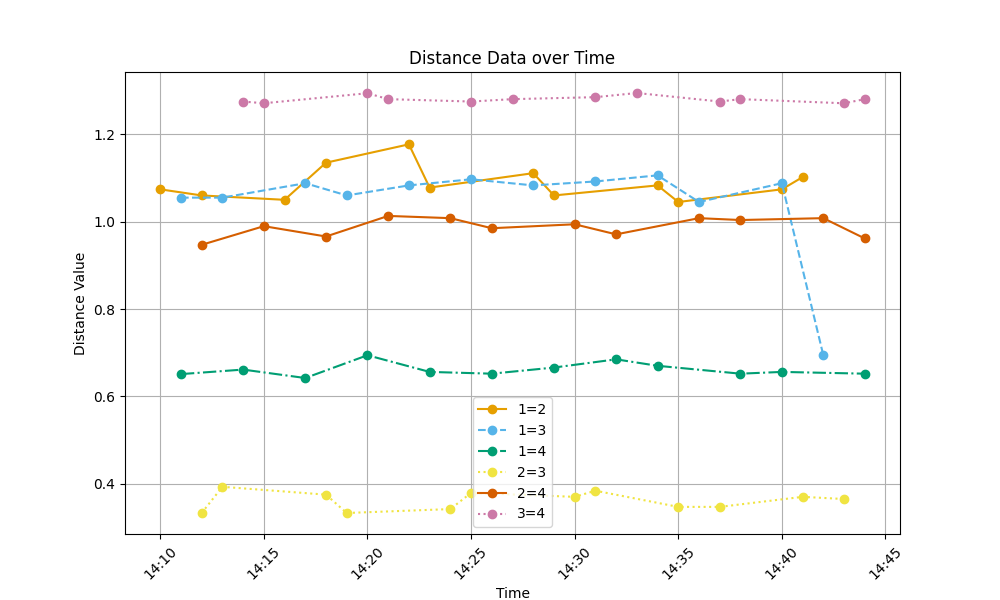
\includegraphics[width=\linewidth]{graphics/exp/exp1_dist_data_plot_1_combined.png}
	\caption{Experiment 1, distance over time, for comined pairs i=j.}
	\label{f:exp1_graphs_dist_combined}
\end{figure}

Since the pairs i-j and j-i report the same data and this fact is consistent in the measurements, they can be combined into one graph.
Figure \ref{f:exp1_graphs_dist_combined} shows the distances over time for all combined pairs i-j and j-i, called i==j.
Graphs like this will be called combined graphs in this report.
Since initiating and reseiving tag can no longer be distinguished, the line colors and types have no assigned meaning.
The two pairs 2=3 and 1=4 corresponding to the two low distances of 0.5m can be seen at the bottom.
The pairs 1=3 and 2=4 that represent the highest distance of 0.94m do not separate and are mixed together with 1=2 and 3=4.\\
Table \ref{tab:exp1_var_distanc} shows the means and variances of the combined tag pairs.
Since the measurements of i=j are the same as j=i, only the upper triangle of the distance-matrix is needed.
The table shows, that the variances are very low for all pairs, except 1=3.

\begin{table}[ht]
\centering
\caption{Statistics of the combined distance measurements between tags for experiment 1}
\begin{minipage}{0.45\textwidth}
\centering
\begin{tabular}{|c|c c c|}
\hline
		& \textbf{Tag-2} & \textbf{Tag-3} & \textbf{Tag-4} \\
\hline
\textbf{Tag-1}    & 0.0.112 & 0.265 & 0.177 \\
\textbf{Tag-2}   &  & 0.368 & 0.824 \\
\textbf{Tag-3}   &  &  & 0.385 \\
\hline
\end{tabular}
\caption*{Mean}
\end{minipage}
\hfill
\begin{minipage}{0.45\textwidth}
\centering
\begin{tabular}{|c|c c c|}
\hline
		& \textbf{Tag-2} & \textbf{Tag-3} & \textbf{Tag-4} \\
\hline
\textbf{Tag-1}    & 0.001 & 0.013 & 0.000 \\
\textbf{Tag-2}   &  & 0.000 & 0.000 \\
\textbf{Tag-3}   &  &  & 0.000 \\
\hline
\end{tabular}
\caption*{Variance}
\end{minipage}
\label{tab:exp1_var_distanc}
\end{table}


\subsection{Conclusion}
\label{s:exp1_conclustion}
The temperature measurement seem to be working as excpected.
All four tags show the same temperature, within a small margin of error.
Variance is low, showing a consistent temperature measurement.\\
Two possible explenations were found for the increase in temperature during the experiment.
One possible explenation is given by the fact, that this was the first experiment performed in the day, and the room temperature was slightly increasing because of the presence of a person, that was not present before.
An alternative explenation is, that the microprocessors proucde heat that was detected.
The fact that the temperature decreased during subsequent experiments, favors explenation one, since their would be no reason for the microcontrolers to stop producing heat.
The decrease itself can be explained, since during setup, the person performing the experiment was close to the sensor, while during the experiment the person stayed in a different part of the room. The dicrease in temperature was smaller, this difference in closness to body heat could explain the difference.


The humidity sensor similarly produced satisfactory results.
All four tags presented the same humidity, only with small margins of error.
The variance is again satisfactory, since it is very small, beeing bellow 0.05%.
The slight increase in humidity can again be explained by this beeing the first experiment of the day, and the person performing the experiment having wet hair from the rain.
This again weakenes the microcontoler heat theory, since rising temperature without adding moisture would only decrease the humidity.\\
The dicrease in humidity in subsequent experiments lacks a clear explenation.
It is a very weak trend, so factors global factors could explain the difference.
Changing weather conditions could account for the difference.
Another proposed explenation arises from the setup of the system.
During setup, each tag was touched repeatedly to put them into position.
The person performing the experiment tends to have clamy hands, that feasably could lead the sensors to detect additional humidity at the beginning of the experiment.\\
Without additional data, no one explenation can be favored over the other. 
Since the decrease in temperature was small, this is not considered a issue for this system.


The Gyroscoping sensor data does not produce any meaningfull result.
The measured orientation of the tags varied widely, while the physical tags stood still.
A possible explenation of this is, that the gyroscope used in the implementation has consistent biases.
Since the angular velocity is evaluated often and then added to the current angle, small errors would acumulate over time.
The time between measurements was 5 minutes and 30 seconds.
A bias of only $\frac{12}{11} \frac{\degreem}{s}$ would correspond to an accumulated error of 360\degree over this timespan.
Since rotational position in inheritly circular, rapping arround at 360 \degree, unless there was no variance next to the bias, the values would end sudo randomly scattered over the range of $[0\degreem , 360\degreem ]$.
The MPU6050 outpus only integers, so any bias at all would have this effect.\\
Be bias hypothoses is additionaly strengthend, by the existance of Tag-2 axis X, that stays at 0 over the course of the measurement.
While this could indicate a faulty sensor, during later experiments using rotational velocity readings, see section\ref{s:exp_5_real_world}, Tag-2 axis X did produce meaningfull results. While this doesn't disproove, that Tag-2 axis X was faulty during this experiment, it makes it more reasonable to assume, that it has a bias of 0. \\
A possible reason for the bias in angular velocity was considered, in the rotation of the earth.
After some consideration, this thesis was dropped, since the angular velocity introduced by the earth would acount for no more than $\frac{1}{240} \frac{\degreem}{s}$ around the X or Y axis, if standing on the equator, where the effect is strongest.\\
The bias explenation seems to be a reasonable and explaines the measured results.
As a consequence, the orientational read has to be considered usless.


The distance measurements have mixed results.
The fact that the tag pairs produce the same same reults is good.
Double sided two-way ranging is used, so during each ranging session both tags conduct single-sided two-way ranging and the results are combined.
It is therefore expected, that the device that initiates the ranging does not matter.\\
The fact that ranging sessions involving Tag-1 occasionaly produce inconsistent results can not directly be explained.
Different locations were used for the experiments and the tags did not always have the same position.
This means that an explanation envolving multi-path effect based on position can be rejected.
The possible explenation envolves a fault on the nRF52840 microcontroler or the DMW3000 shield. 
Since the final calculation relies on the timestamps recorded during the ranging, a possible explenation would be, that the clock of the nRF52840 sometimes faults, or that there is an issue with the clock line of the SPI connection.\\
The fact that the resulting distances are wrong is troublesome.
The proposed design that would calculate the position by solving a quadratic program relies on somewhat accurate distance measurements.
The likely reason for the distance measurements producing wrong results is the simplified calibration, that was used for the $d_{rx}$, $d_{tx}$ values, see Section \ref{ss:two_way_ranging}.
The fact that the distances still sort themself into high and low values correctly indicates, that some calibration has worked, but it is not granular enough to work for small distances.\\
The distance measurements can currently not be used to build a model of the tag positions.
If they can be used to detect movement can not be determined by the static experiment and requires the introduction of movement, see Experiment 4 \ref{s:exp4}


\section{Experiment 2: Temperature}
\label{ss:exp_2}
The four tags were placed in the same 80 cm by 50 cm rectangle as in experiment one.
One tag placed on a elevated surface, 4 cm above the table.
Under the tag seven candles were placed (see figure TODO, Bild einfügen).
Next to the tag two thermometers detectors were placed.
Each tag was turned on sequentially and given enough time to establish the network.
The phone then was connected to one tag.
The max Temperature parameter in the app was changed to 35\degree C.
After 20 minutes the candles were lit.
The experiment was then left alone for another 30 minutes.
The independent thermometers were filmed during the process, to allow for later review and comparesment.
The goal of experiment 3 was to test the temperature detection capabilities of the system.

\subsubsection{Results}
\label{ss:exp_2_result}
Experiment two introduced heat-sources the system.
Since the main setup was the same as experiment 1 \ref{ss:exp_1_result}, many of the findings are the same.
In this section, only differences in results are discussed.
If a metric is not measioned, one can assume it behaved the same as for experiment 1  (see section \ref{ss:exp_1_result}).

\begin{figure}[ht!]
	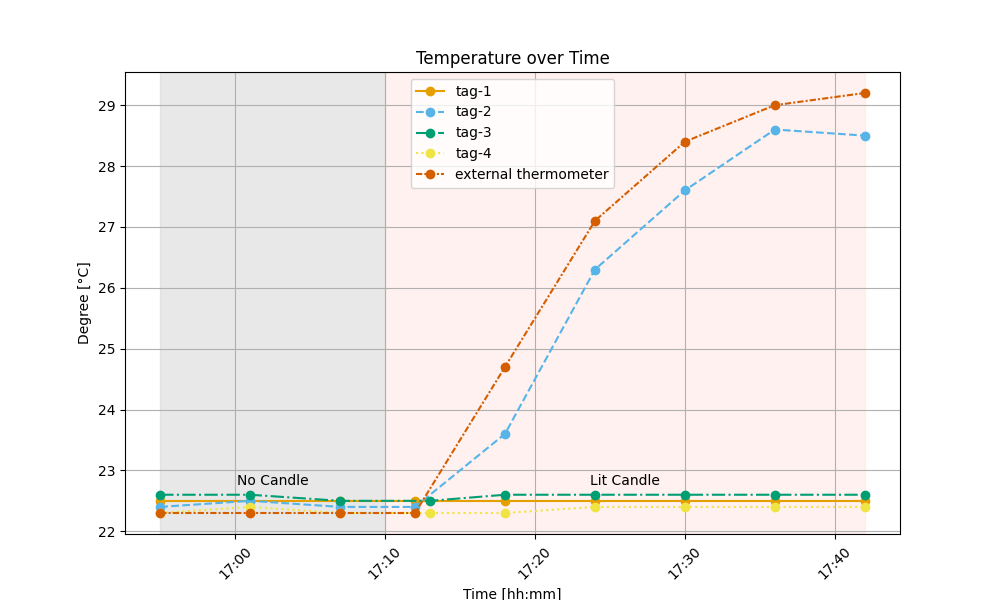
\includegraphics[width=\linewidth]{graphics/exp/exp3_temp_plot_1.png}
	\caption{Experiment 3, temperature over time, mith external measurement added.}
	\label{f:exp3_graphs_temp}
\end{figure}

The progression of the external thermoeter and the internal temperature sensor can be seen in figure \ref{f:exp3_graphs}.
The candles, that functioned as the heat source, were lit at 15.10.
During the next measurement of tag 2, at 15.12, both the external thermoeter and the temperature sensor on tag 2 had not yet registered any change, remaing at 22.4 \degree C.
The extrenal thermometer started rising 1 minutes later, at 15.13.
During the next measurement at 15.18, the temperature-sensor registered a slightly increased temperature of 23.6 \degree C, while the external thermometer registered 24.7 \degree C.
During the next measurement at 17.24 the tag reported 26.3 \degree C while the thermometer showed 27.1 \degree C. 
The measured temperature of the external thermometer keeps klimbing faster than the internal temperature sensor, until the end of the experiment, as seen in Figure \ref{f:exp3_graphs_temp}.
Their distance nether exeeds 1 \degree C and gets smaller towards the end of the experiment.
The other tags do not report any significant change in temperature.

\begin{figure}[ht!]
	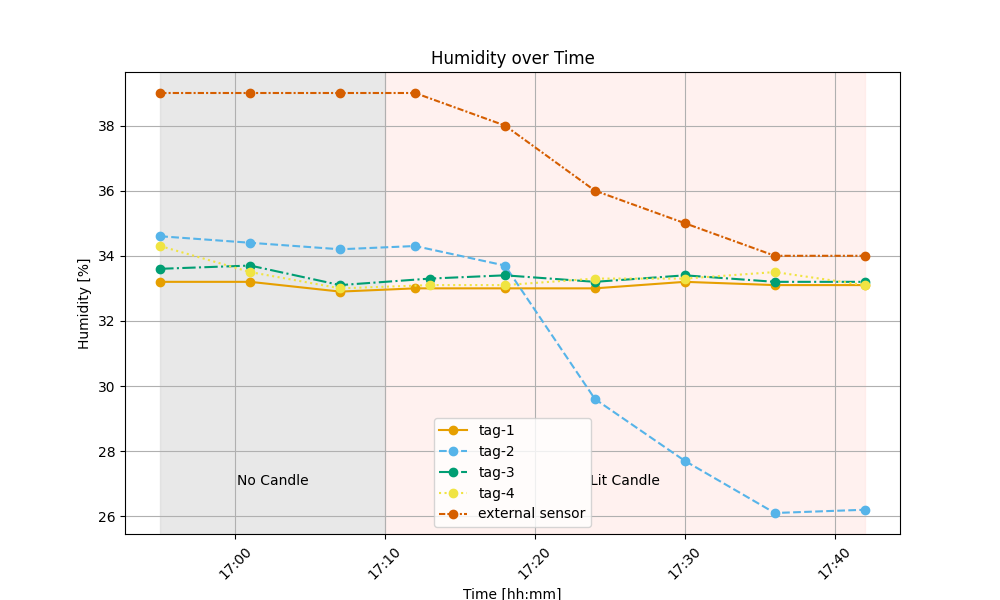
\includegraphics[width=\linewidth]{graphics/exp/exp3_hum_plot_1.png}
	\caption{Experiment 3, humidity over time, with external measurement added.}
	\label{f:exp3_graphs_hum}
\end{figure}


Experiment 3 was intended to test the temperature and not the humidity.
Luckily, the external thermoeter also included a humidity sensor, that could retroactivly be used for evaluation.
Figure \ref{f:exp3_graphs_hum} shows the humidity over time, with a added humidity sensor added to the graph.
Since the external humidity sensor was initialy not intended to be used, it is not perticulalry precise and does not display any digits after the decimal point.
The humidity sensor consitently shows a much higher humidity than the one on the tag.
Once the experiment starts at 15.10, the humidity behaves inversly to the temperature and starts falling.
This happens with the external sensor as well as the internal one in parallel.
The registered values plato at 34\% for the external and 26\% for the internal sensor.
The other tags do not report any significant change in humidity.


\section{Experiment 3: Gyroscope}
\label{s:exp_3}
Again all for tags were placed on a 80 cm by 50 cm rectangle.
Each tag was turned on sequentially and given enough time to establish the network.
The phone then was connected to one tag.
After 20 minutes one tag was turned by 90\degree counterclockwise.
The experiment then ran for another 30 minutes.
The goal of experiment number 4 was to test the detection of unwanted rotations.
Experiment four was repeated with, with the gyro sending the angular velocity for all axes instead of the current position.

This experiment was performed in two differing manners.
The orirentational read was originaly the only implementation for the gyroscope.
After experiments one to four were evaluated, the lack of usefull results from the gyroscope readings prompted a redesign of the sensor.
This resulted in the development and implementaiton of the angular velocity read.
Experiment 3 was repeated with the angular velocity read of the gyro.\\
For the orientational read, the maximal allowed angular difference was set to 30\degree.
For the angular velocity read, the maximal allowed angular velocity was set to 100 $\frac{\deg}{s}$.


\subsection{Reults orientational read}
\label{ss:exp_3_result}
Experiment 3 was intended to check the functionality of the gyroscope.
Temperature and humidity behaviour was the same as in the static experiment \ref{ss:exp_1_result}.
As already seen in during the evaluation of experiment 1, the gyroscope does not work as planned.
Figure \ref{f:exp4_graphs_gyro} shows the values of the gyro over time.
Tag 1 was rotated by 90\degree  at 22.25 around the Z axis.
Their is no disernable change in the output of the gyro during or after this process.

\begin{figure}[ht!]
	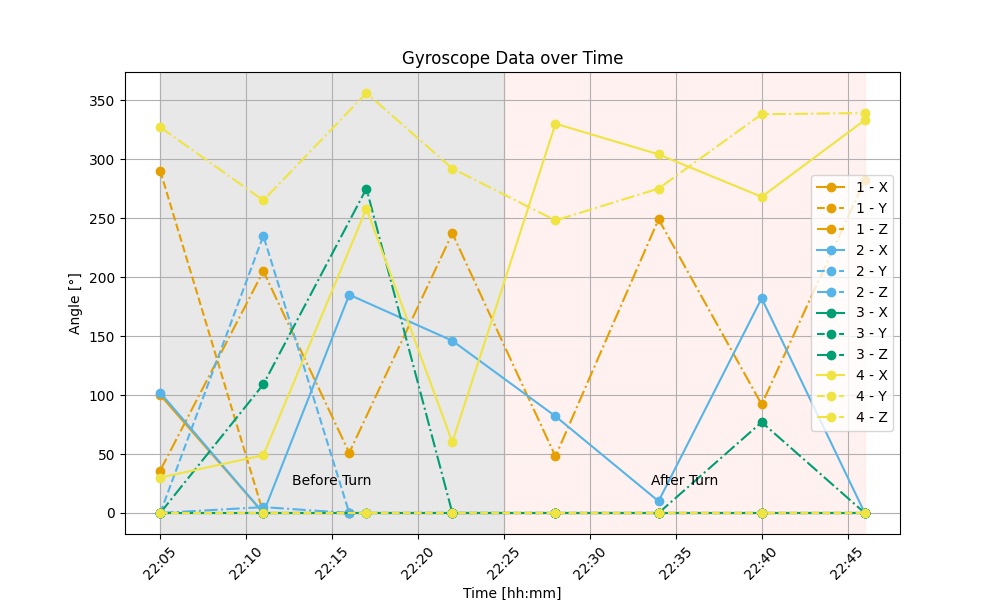
\includegraphics[width=\linewidth]{graphics/exp/exp4_gyro_data_plot_1.png}
	\caption{Experiment 4, gyroscope over time.}
	\label{f:exp4_graphs_gyro}
\end{figure}
Figure \ref{f:exp4_graphs_dist} shows the distances of the tags during the experiment.
Before the event, all tags are in a stable state.
As in experiment 1 \ref{ss:exp_1_result} the distances do not represent what is physically happening.
After the tag is turned at 22.26, all measurements involving tag 1 change, and becomming stable again afterwards.
This can be bit hard to see, since "2-1" and "3-1" have an outlier measurement right before and "1-2" right after.
Distance 1 to 2 and 1 to 3 changes between 0.2 and 0.3 meters and distance 1 to 4 changes by arround 0.4 dm.

\begin{figure}[ht!]
	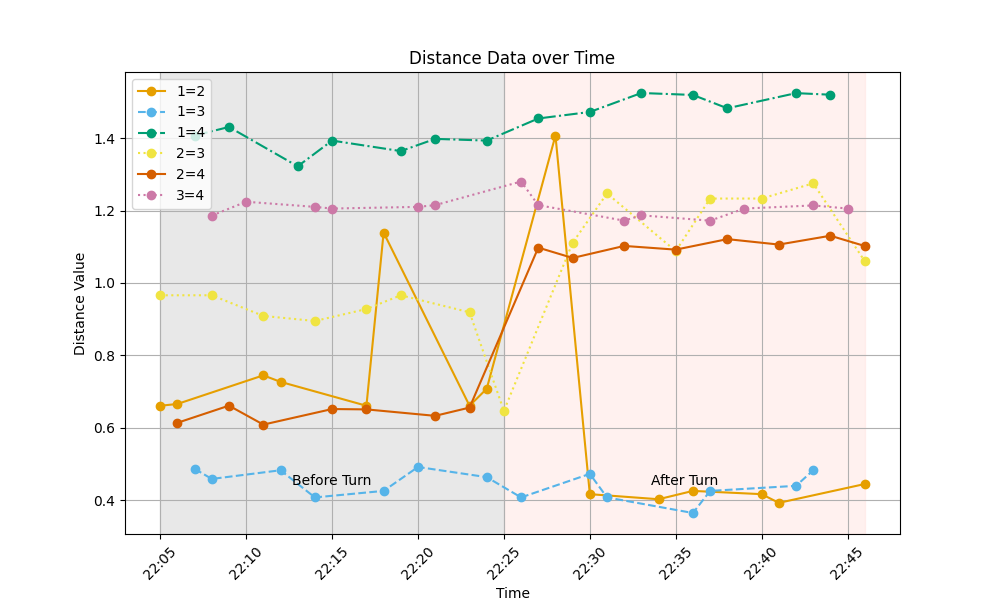
\includegraphics[width=\linewidth]{graphics/exp/exp4_dist_data_plot_1.png}
	\caption{Experiment 3, gyroscope over time.}
	\label{f:exp4_graphs_dist}
\end{figure}


\subsection{Reults angular velocity read}
\label{ss:exp_3_result}
The experiment was started at 10:01 and was terminated 10.40.
Tag 2 was turned at 10.18 by 90\degree clockwise around the Y axis by hand.
Figure \ref{f:exp4_graphs_gyro_2} shows the angualr velocity of all tags during the experiment.
The measurements of a i around axis v will be labeled as i-v.
All axises of Tag-2 are shown in blue, with the angular velocity around the X axis 1-X beeing a filled line, around the Y-Axis a dashed line and around the Z axis beeing dashed and dotted.
The Y axis of figure\ref{f:exp4_graphs_gyro_2} is displayed using a log-scale, to better show the low values.
The time before the trun has a gray backgroudn, while the time after the turn is displayed with a red background.


Tag-2 has constant angular velocity for all three measurements before the turn.
2-X is $12\frac{\degreem}{s}$, 2-Y is between $14\frac{\degreem}{s}$ and $17\frac{\degreem}{s}$  and 2-Z is a constant $20\frac{\degreem}{s}$ before the turn.
The first measurement after the turn reports angular velocities of $445\frac{\degreem}{s}$, $6322\frac{\degreem}{s}$ and $716\frac{\degreem}{s}$ for axis X,Y and Z.
Afterwards the values return back to their original values.
2-X is $13\frac{\degreem}{s}$, 2-Y is $14\frac{\degreem}{s}$ and 2-Z $20\frac{\degreem}{s}$, all constant measurements.

\begin{figure}[ht!]
	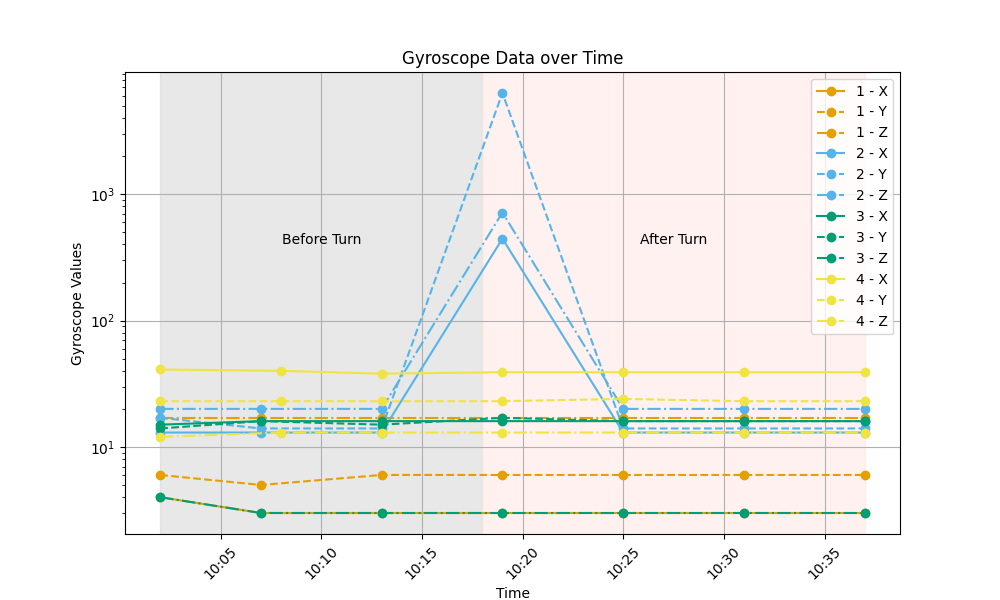
\includegraphics[width=\linewidth]{graphics/exp/exp4_2_gyro_data_plot_2.png}
	\caption{Experiment 3, gyroscope over time, using the angular velocity read.}
	\label{f:exp4_graphs_gyro_2}
\end{figure}

Tag-1, Tag-3 and Tag-4 are in orange, green and yellow respectivly.
They all keep a measurements with minimal fluctuation.
Table \ref{tab:gyro_mean_2} shows the mean values and variances of all tags and all axes.
Tags-1 has no variance that exceeds 0.143, with 1-Z even showing a constant value over all seven measurements, leading to a variance of zero.
Tag-3 and Tag-4 both have two axes with variances of 0.143 and one axis with a variance of 0.905.
The mean values of Tag-1, Tag-3 and Tag-4 are in the reange of $3\frac{\degreem}{s}$ and $40\frac{\degreem}{s}$, with five falling into the range of $15\frac{\degreem}{s}$ to $25\frac{\degreem}{s}$.
Tag-2 has variances between 740 and 16128.

\begin{table}[h!]
\centering
\caption{Summary of Gyroscope Data: Means and Variances of X, Y, Z Axes}
\begin{tabular}{c|c c c|c c c|}
\hline
\textbf{tag} & \textbf{mean x} & \textbf{mean y} & \textbf{mean z} & \textbf{var x} & \textbf{var y} & \textbf{var z} \\
\hline
\textbf{tag-1} & 3.143 & 5.857 & 17.000 & 0.143 & 0.143 & 0.000 \\
\textbf{tag-2} & 23.3 & 41.3 & 68.0 & 741 & 5024 & 16128 \\
\textbf{tag-3} & 15.857 & 15.714 & 3.143 & 0.143 & 0.905 & 0.143 \\
\textbf{tag-4} & 39.286 & 23.143 & 12.857 & 0.905 & 0.143 & 0.143 \\
\hline
\end{tabular}
\label{tab:gyro_mean_2}
\end{table}


Figure \ref{f:exp4_graphs_dist_comb_2} shows the combined distance graph of experiment 3 using angualr velocity read.
The distances 1-2, 1-3, 1-4, 2-3 and 2-4 stay in a similar range over the whole experiment.
Table \ref{tab:exp4_var_distanc} shows the mean and variance of the combined distance measurements.
The variance in measured distances 1-2, 1-3, 1-4, 2-3 and 2-4 are all below one milimeter.
The measured distances are between 0.39m and 0.87m.
The measured distance 3-4 behaves very differently.
It is bigger than all others, with 1.18m.
It also has a comparatavly high variance of 0.05m.
Its lowest measurement is the first measurement after the turn.
Looking at the split distance-measurement 3-4 in figure \ref{f:exp4_graphs_dist_split_3_4} shows, that the change in distance comes mainly from the measurements originating from tag 3.
Distance measurements from Tag-3 to Tag-4 have a variance of 0.074m, while measurements from Tag-4 to Tag-3 have a variance of 0.014m

\begin{figure}[ht!]
	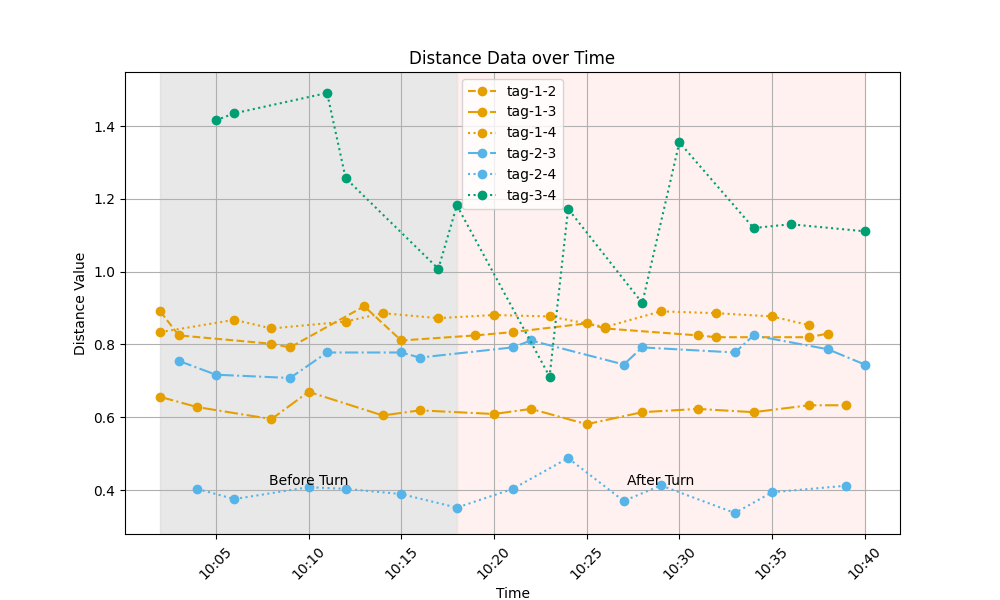
\includegraphics[width=\linewidth]{graphics/exp/exp4_2_dist_combined_2.png}
	\caption{Experiment 3, combined distance over time, using angular velocity read.}
	\label{f:exp4_graphs_dist_comb_2}
\end{figure}

\begin{table}[ht]
\centering
\caption{Statistics of the combined distance measurements between tags for experiment 3 with angular velocity read}
\begin{minipage}{0.45\textwidth}
\centering
\begin{tabular}{|c|c c c|}
\hline
  & 2 & 3 & 4 \\
\hline
1    & 0.0.834 & 0.622 & 0.868 \\
2   &  & 0.770 & 0.396 \\
3   &  &  & 1.177 \\
\hline
\end{tabular}
\caption*{Mean}
\end{minipage}
\hfill
\begin{minipage}{0.45\textwidth}
\centering
\begin{tabular}{|c|c c c|}
\hline
  & 2 & 3 & 4 \\
\hline
1    & 0.001 & 0.001 & 0.000 \\
2   &  & 0.001 & 0.001 \\
3   &  &  & 0.049 \\
\hline
\end{tabular}
\caption*{Variance}
\end{minipage}
\label{tab:exp4_var_distanc}
\end{table}

\begin{figure}[ht!]
	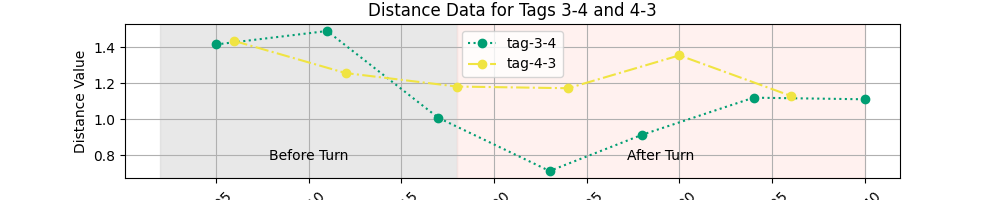
\includegraphics[width=\linewidth]{graphics/exp/exp4_2_gyro_split_distance_3_4.png}
	\caption{Experiment 3, split distance measurement between Tag-3 and Tag-4 over time.}
	\label{f:exp4_graphs_dist_split_3_4}
\end{figure}

\section{Experiment 4: Distance}
\label{ss:exp_4}
The same 80 cm by 50 cm rectangle setup was used.
The tags were turned on sequentilay, giving them enough time to build the network.
The phone was connected to one tag.
The max distance parameter was set to 20 centimeter.
After 20 minutes, one tag was moved parallel to the shorter rectangle line about 20 cm towards the tag on the next corner.
The system was then left resting for another 30 minutes.
The goal of experiment number 5 was to test the detection of unwanted movement.

\subsection{Results}
\label{ss:exp_4_result}

Experiment four was intended to test the distance measurement capabilities of the setup.
Temperature and humidity and gyro behave as they do in experiment 1 \ref{ss:exp_1_result}.
They will not be discussed for this experiment.

\begin{figure}[ht!]
	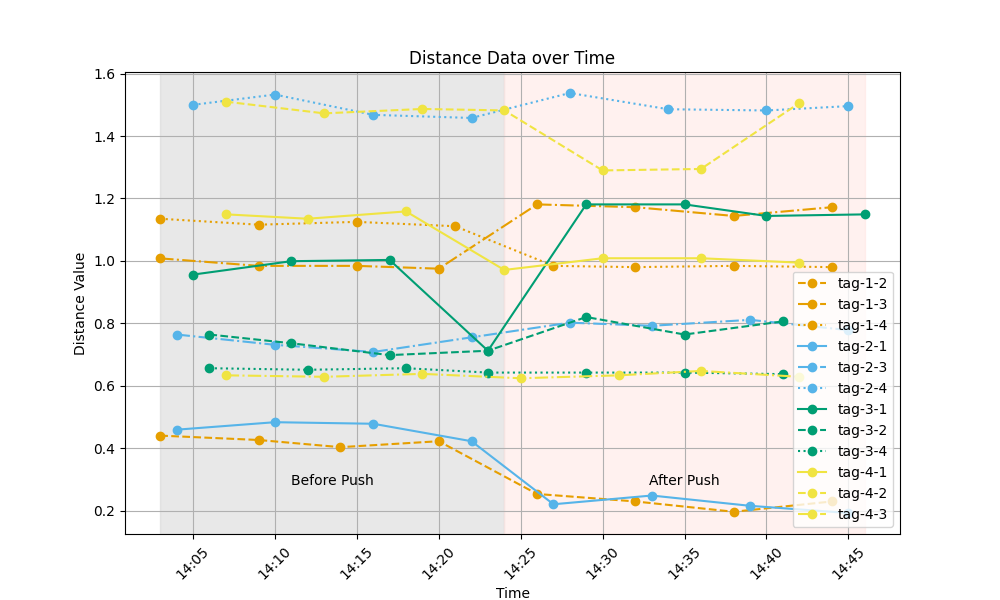
\includegraphics[width=\linewidth]{graphics/exp/exp5_dist_data_plot_2.png}
	\caption{Experiment 5, distance over time.}
	\label{f:exp3_graphs_dist}
\end{figure}

Figure \ref{f:exp5_graphs_dist} shows the measured distances of the 4 tags over time.
As in the static experiment, the measured distances of two devices are similar and mostly stable, before any movement is introduced.
As in experiment 1 the values reported are not correct.
At 14.24 tag 1 is moved by 0.23 meters toward tag 2.
The measured distances to tag 3 increases while the distance to tags 2 and 4 dicreases.
This represent what is happening in reality, since tag 1 is now closer to tag 2 and 4 and further away from tag 3 as before.
The difference in distance is roughly 0.2 meters for tag 2.
This is correct, since tag 1 was moved about that distance towards tag 2.
The measurements show tag 4 now 0.15 meters closer to tag 1.
The effect on tag 4 should be notissable but not as large as it is.
Since the tag moves lateraly towards tag 4, the difference should only be 0.11 meters.
The same is true for tag 3.
The difference in measured distance between 1 and 3 is between 0.15 and 0.2 meters. 
This is too large for the difference a latteral move, it should only be a 0.02 meters difference.
Their is also a small increase in the distance between tags 2 and 3, but which starts before tag 1 was moved.


\section{Experiment 4: Distance}
\label{s:exp_5_real_world}


\section{Experiment 5: Real World experiment}
\label{s:exp_5_real_world}